\documentclass[addpoints, 12pt] {exam}
\usepackage{graphicx}
\usepackage{amsmath}
\bracketedpoints
\pagestyle{headandfoot}
\runningheadrule
\firstpageheader{Math 112}{Written Homework 7}{Due March 1st 2024}
\runningheader{Math 112}{ Page\; \thepage\; of\; \numpages}{Written Homework 7}
\firstpagefooter{}{}{}
\runningfooter{}{}{}
\setlength\answerskip{2ex}
\setlength\answerlinelength{1.5in}
\begin{document}

\begin{center}
\fbox{\fbox{\parbox{5.5in}{\centering
Directions:\\Please only put your final, well written solutions, in the space provided.\\ Give exact answers (simplified radicals or fractions).\\If you use additional paper clearly label the question and upload pages after the question page.\\Use complete sentences and explain your reason as much as possible.\\There are \numquestions\,  questions and \numpoints\, points total
}}}\end{center}
\vspace{0.1in}
\makebox[\textwidth]{Name:\enspace\hrulefill}
%\qformat{Question \thequestion \dotfill \thepoints}%

\begin{questions}
\question 
\begin{parts}
\part[2] Please provide a clear definition for the statement: \(y\) is a function of \(x\) \vspace{1in}
\part[4] Using the graph provided, sketch the inverse of the function shown in red.\newline

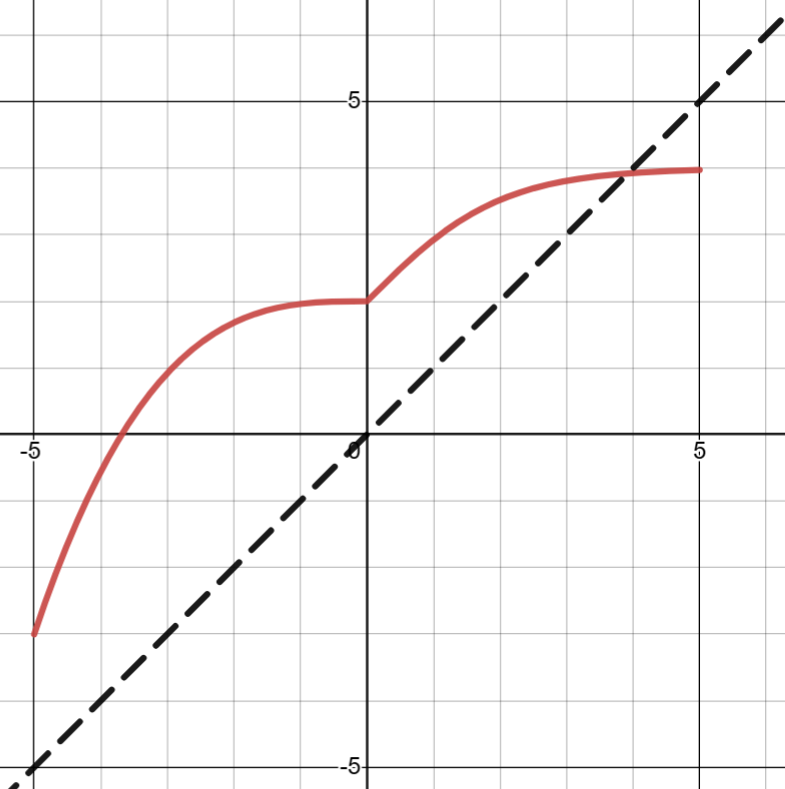
\includegraphics[scale=0.25]{sketchinverse}

\part[4]Provide a short argument on whether or not the graph of the function \(f(x)\) below has an inverse.\newline
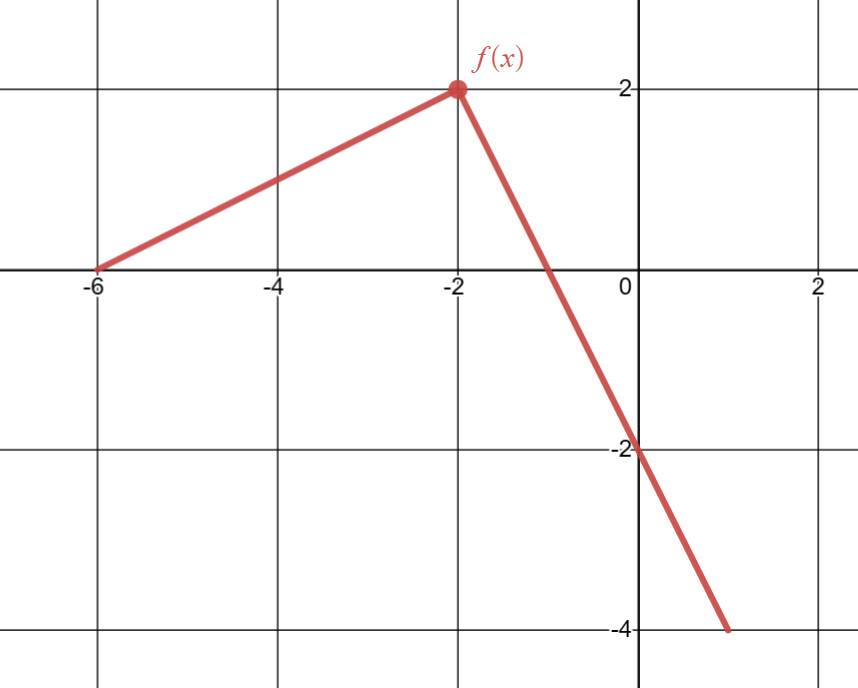
\includegraphics[scale=0.25]{isinvertible}
\end{parts}
\newpage
\question Consider the function \(D = f(p) = 100-4p\) which represents the demand for a particular hairgel when the price is \(p\) dollars.
\begin{parts}
\part[4] Determine the inverse of this function. Show your work and the final inverse function.\vspace{1in}\answerline
\part[2] Describe, in your own words, the contextual meaning of this inverse function.\vspace{1in}
\part[2] The point \((60,10)\) lies on the graph of the \emph{inverse} function. Describe what this point represents in the context of this problem.\vspace{1in}
\part[2] What price will result in a demand for 50 units the hairgel?
\end{parts}
\newpage
\question In a hospital, a patient is presenting with an unknown illness. In order to rule out different diagnoses, the patient's mouth and nose are swabbed and a bacterial cultural is grown in a petri dish over the course of the next ten hours. The population of the bacteria on the dish is found to follow the following model: \[P=f\left(t\right)\ =\frac{100t+23}{5+7t},0\leq t\leq 10\;\;\;\]Where \(P\) is the population in thousands and \(t\) is the time in hours.
\begin{parts}
\part[5]Determine the inverse of this function, \(t=f^{-1}(P)\). Show all your steps.\vspace{2.5in}\answerline
\part[3] Give both the numerical answer, rounded to the nearest tenth, and the practical meaning of \(f^{-1}(12)\).\vspace{1in}\answerline
\part[2] In order to properly identify the bacterial strain, there needs to be at least ten thousand bacteria present in the dish. How long will the lab need to wait until there are at least that many bacteria? \vspace{1in}\answerline
\end{parts}\newpage
\question Murphy invests \(\$750\) into a bank account that earns a fixed \(1.25\%\) compounded annually. This type of investment is given by the equation \[A=f(t) = 750(1.0125)^t\]
\begin{parts}
\part[1]What is the contextually appropriate domain for this function?\answerline
\part[1]What is the contextually appropriate range of this function?\answerline
\part[1]Using Desmos (or a graphing utility of your choice) graph this function. You will need to pick a window that provides a reasonable visualization of the function given the domain/range you chose. Include a screenshot of your graph, either as a separate page or included below.\newpage
Question 4 cont'd
\part[1]Provide a brief explanation why this function \emph{does} have an inverse.
\vspace{2in}
\part[2]Provide a brief description of what the inverse function would mean in the context of this problem.\vspace{2in}
\part[1]What is the domain of the inverse function?\answerline
\part[1]What is the range of the inverse function?\answerline
\part[2]When will Murphy have \(\$2000\) in their account if they only rely on the interest they earn? Explain how you come to your answer.\vspace{1.5in}\answerline
\end{parts}
\newpage
\question \emph{This is not for credit nor is it anoynymous. However, if you would like to answer any of the following, your feedback would be appreciated.}

How is the semester going for you so far? What are you doing well? In what ways can you improve?\vspace{3in}\newline
How is your experience with the online course? What am {\bf I} (the instructor) doing well? What are the TA's doing well? What can we do to improve? \vspace{3in}\newline Thank you for you thoughtful feedback.
\end{questions}


\end{document}